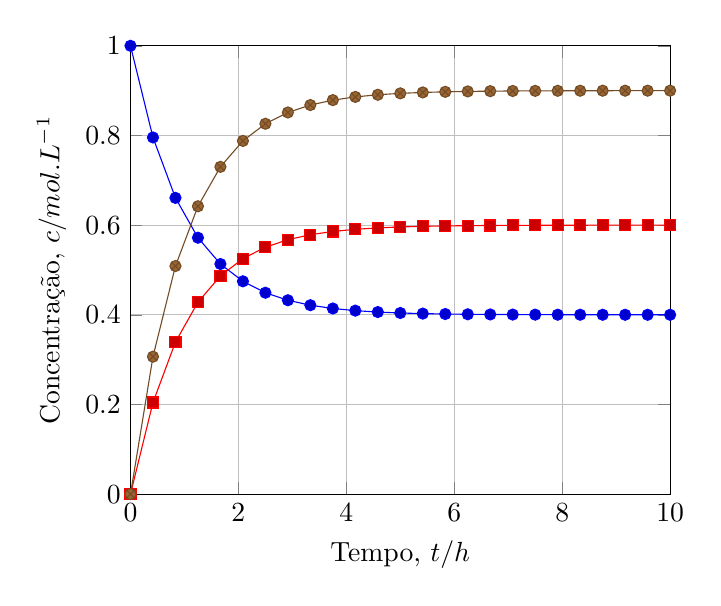
\begin{tikzpicture}
    \begin{axis}[
        xlabel={Tempo, $t/\unit{h}$},
        ylabel={Concentração, $c/\unit{mol.L^{-1}}$},
        grid=both,
        xmin=0, xmax=10,
        ymin=0, ymax=1,
        domain = 0:10,
    ]
    \addplot {
        0.4 + 0.6*exp(-x)
    };
    \addplot {
        0.6*(1 - exp(-x))
    };
    \addplot {
        0.9*(1 - exp(-x))
    };
    \end{axis}
\end{tikzpicture}